\documentclass{article}
\usepackage{amsmath}
\usepackage{graphicx}
\begin{document}
\title{Problem Redone: Question 8}
\author{Ana Bhattacharjee}
\date{\today}
\maketitle

\begin{center}
  \begin{figure}[!htbp]
    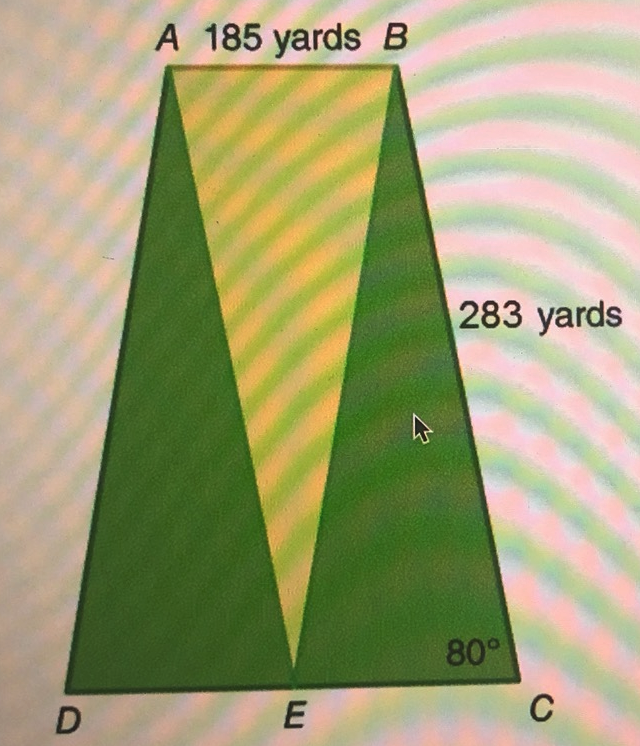
\includegraphics[width=0.90\columnwidth]{new_image}
    \caption{Land}
  \end{figure}
  Since the three isoceles triangles are congruent, we can define each isoceles triangle with the following dimensions:
  \begin{figure}[!htbp]
    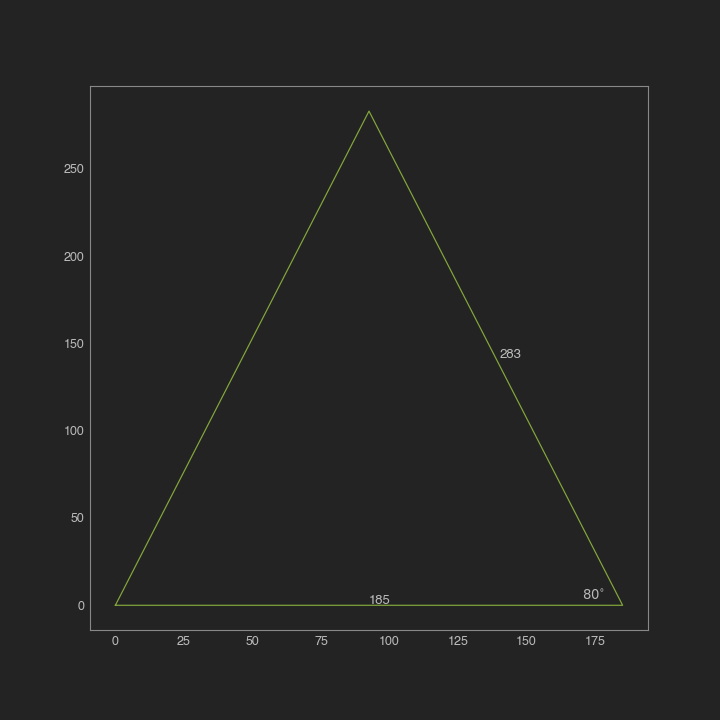
\includegraphics[width=0.90\columnwidth]{triangle}
    \caption{Isoceles Triangle}
  \end{figure}
  Now that we have three equivalent isoceles triangles, we know that the farmer wants to plant vegetation in the area containing two of these triangles. In order to do this, we need to use the formula $ A = \frac{1}{2}ab*sin(C)$ to find the area of one isoceles triangle. Since the area of each green isoceles triangle will be the same, we can simply do the following:
  \begin{align}
    A = 2*\frac{1}{2} ab*sin(C) \\
    A = ab*sin(C) \rightarrow 185 (283) sin(80) \\
    A = 52355 sin(80) \\
    A \approx 51559.61 \text{ yd}^2
  \end{align}
\end{center}

\end{document}
